\section*{The Four Data Science Core Classes}

This course is one of the four data science core courses but it does not cover any typical \qu{data science} topics. Instead, it is designed to provide theoretical skills for Math 341 and 343. Math 340 and 342W are designed to be standalone courses and the other two courses rely on topics covered therein. Thus there is an order the classes need to be taken. Below are two plans, the first is over two semesters and hence it is not \emph{not recommended} as it will be a \emph{very} heavy workload. The second is over four semesters and it is the recommended plan as I believe it will allow students to absorb the material more effectively:

\begin{figure}[htp]
\centering
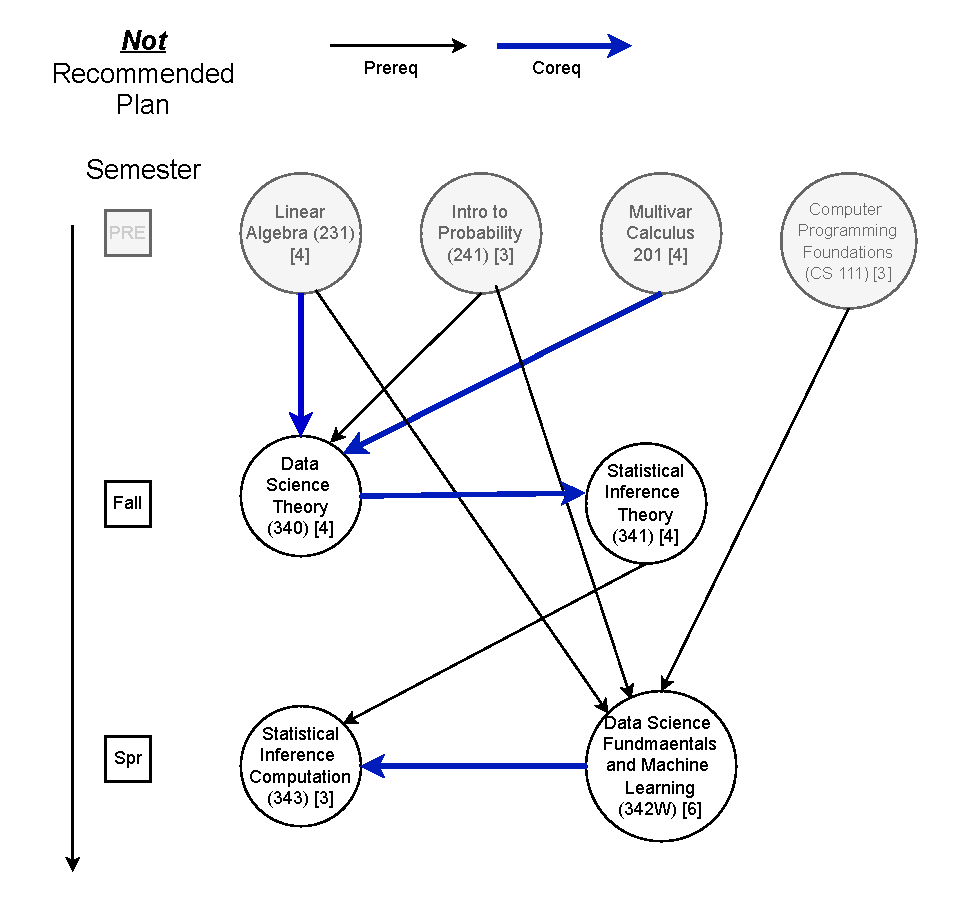
\includegraphics[width=6in]{../../syllabi/not_recommended_plan.pdf}
\label{fig:not_recommended}
\end{figure} 

\begin{figure}[htp]
\centering
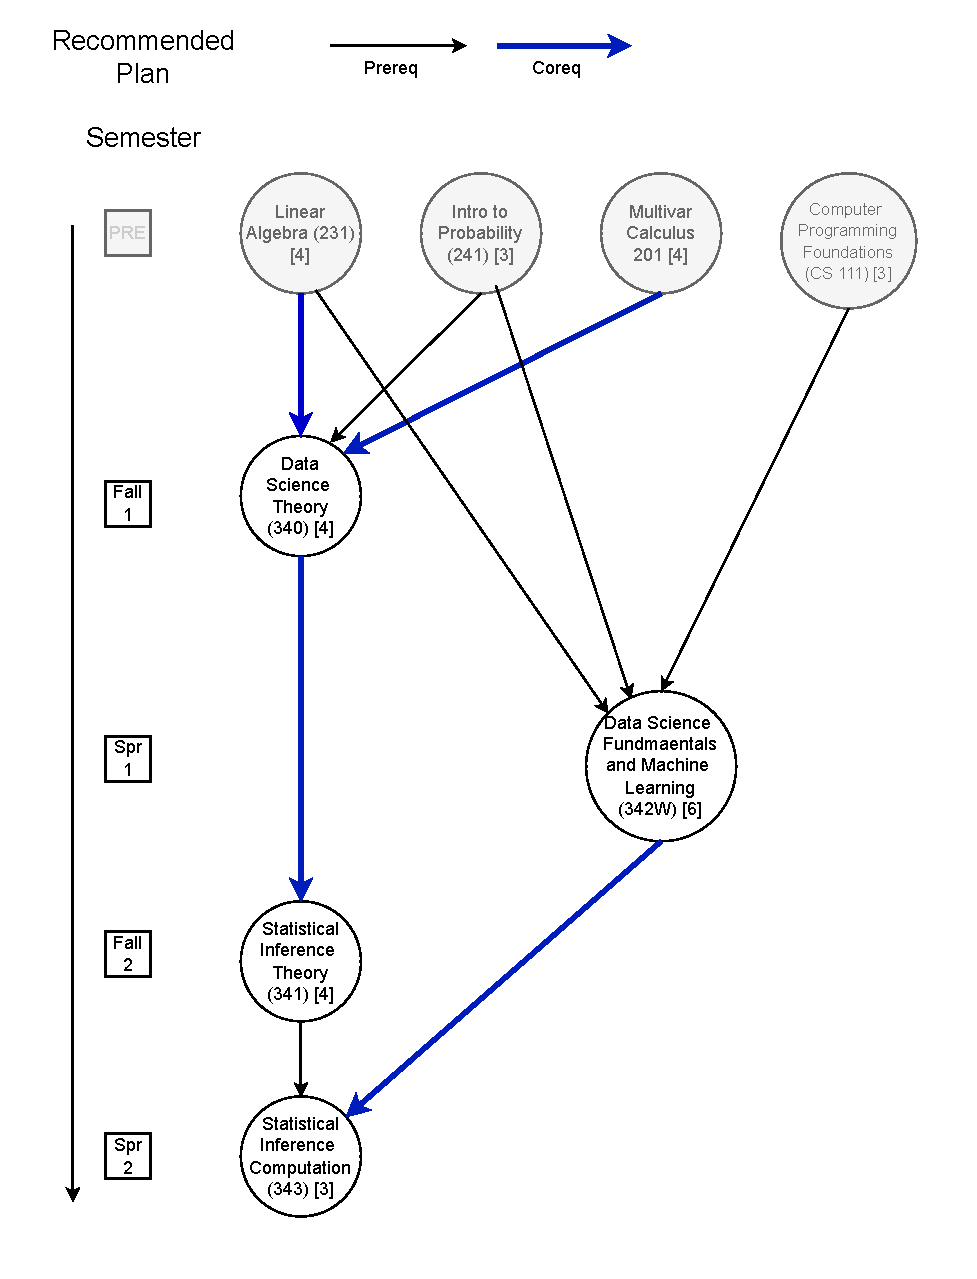
\includegraphics[width=6in]{../../syllabi/recommended_plan.pdf}
\label{fig:recommended}
\end{figure} 